\documentclass[11pt]{article}


\usepackage{geometry}
\geometry{letterpaper}


\usepackage{doc}
\usepackage{cite}
\usepackage[margin=1cm]{caption}


\usepackage{url}


\usepackage{graphicx}
\usepackage{epstopdf}
\DeclareGraphicsRule{.tif}{png}{.png}{`convert #1 `dirname #1`/`basename #1 .tif`.png}


\title{Usability of Modern Display Technologies}
\author{Rachel Rivera}
\date{October 21, 2014}


\begin{document}


\maketitle


\abstract{
This study aims to examine how interaction design concepts specifically map to the usability of modern display technology. This paper discusses the limitation of the lack of tactile feedback for touchscreen devices as well as how this limitation affects usability. This paper examines some current proposed solutions for making touch surfaces truly tangible. This limitation and each proposed solution has a variety of implications with respect to learnability, efficiency, satisfaction and errors. 

}


\pagebreak
\tableofcontents



\pagebreak


\section{Introduction}
\label{introduction}

Electronic screens are devices through which information is transferred between the user and the interface. Although electronic displays have been around for roughly a century,\footnote{One of the earliest electronic displays, the cathode ray tube (CRT),  was first made commercial in 1922.\cite{Cathode}} they are still diversifying in a multitude of ways to tackle the limitations that have presented themselves over the years.\cite{Eisenberg} Screen devices have been changing in size, shape, flexibility, and resolution in order to improve usability for specific tasks. For example, \textit{focus plus context screens}, which are wall-size low-resolution displays with an embedded high-resolution display region, are currently a proposed solution to working with visual documents too large to fit standard screens.\cite{Baudisch} Another kind of screen that is emerging is the \textit{BiDirectional (BiDi) Screen}, which is a thin, depth-sensing liquid-crystal display (LCD) that allows for 3D interaction using light fields.\cite{Hirsch} 

 Though each kind of screen has its merits, this study will focus exclusively on touch sensitive screens. In a study from Link\''{o}ping University, researchers articulated how ``interaction on touch sensitive screens is literally the most `direct' form of HCI, where information display and control are but one surface.''\cite{Albinsson} Though it is clear that a connection between modern touchscreen devices and the field of interaction design exists, this study aims to investigate exactly \textit{how} interaction design concepts specifically map to the usability of touch screens. 


\section{Background/ Prior Work/ Literary Review}
\label{background}
\subsection{Limitations/Proposed Solutions}
There exists a fair amount of previous work pertaining to the usability of touch sensitive screens. The literature often evaluates usability by examining the limitations of these screen devices, as well as the proposed solutions for the limitations. One frequently discussed limitation is how typing on flat surfaces---with no physical keys to guide the fingers---requires heightened visual attention. A study by Hussain Tinwala and Scott MacKenzie suggests that since the visual demand on the user is increased, concentration is diverted from the thoughts being expressed. \cite{Tinwala:2010:ETE:1868914.1868972} The lack of tactile features not only diverts attention from thoughts being expressed, but moreover, it makes the devices difficult to use for Individuals with Blindness or Severe Visual Impairment (IBSVI). A study from Virginia Polytechnic Institute and State University examined how touch screens---even those that include features such as  \textit{VoiceOver}\footnote{\textit{VoiceOver} for OS X tells users what is on the screen and walks users through actions.\cite{VoiceOver}}---do not provide sufficient support for IBSVI. These users were only able to ``develop a spatial mental model for the interface or the screen through dead reckoning'' since there was an ``absence of any landmark other than the boundary of the device.'' \cite{El-Glaly:2013:TTF:2460625.2460665} 

One purposed solution to this limitation is the use of a tactile overlay. (See Figure~\ref{tactile-grid}) One such overlay was recently developed by researchers specifically to help IBSVI engage their spatial cognition, perception, and sensing resources while interacting with touch screens.  \cite{El-Glaly:2013:TTF:2460625.2460665} The tactile overlay covers the touch device screen and IBSVI can use the tactile patterns of the overlay to locate the text, icons, or buttons in the touch device interface. A study examining the efficacy of this physical overlay illustrated that IBSVI who used it were generally more efficient than those using voice-over technology or `trail-and-error' exploration. \cite{El-Glaly:2013:TTF:2460625.2460665}

\begin{figure}[ht]
\centering
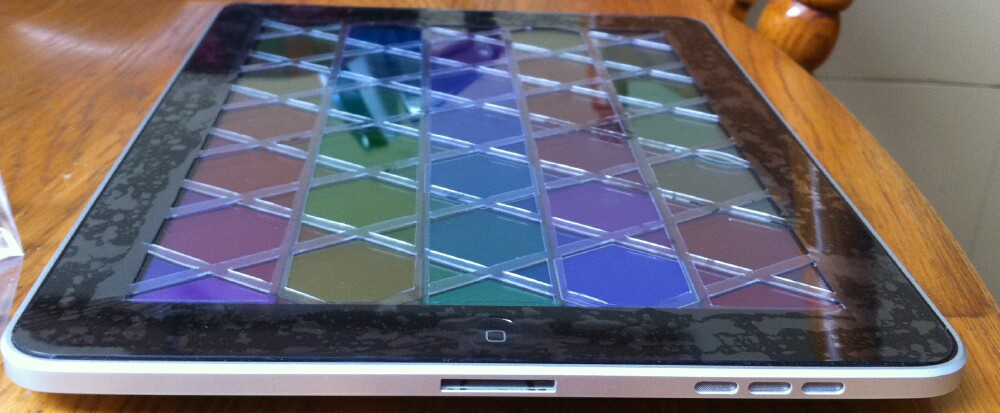
\includegraphics[width=3in]{TactileGrid.jpg} 
\caption{A Tactile Grid}
\label{tactile-grid}
\end{figure}

Another limitation of touchscreen devices that is examined in the literature is how the human finger as a pointing device has ``very low resolution.''\cite{Albinsson} With mobile touch screens in particular, research has illustrated the difficulty in pointing at targets that are often smaller than the width of the user's finger. A notable technique was created by Schneiderman, Sears, and colleagues to specifically address this problem.\cite{Sears} Their basic technique provides a cursor above the user's finger tip with a fixed offset when touching the screen. The user drags the cursor to a desired target and then lifts the finger to select the targeted object. Although this technique generally allowed a user to perform precise movements with less errors, the user's efficiency tended to suffer.\cite{Sears}

Many studies have purposed using a stylus (pen) to interact with touch screens instead of using a bare finger. A stylus has better ``resolution'' than a finger tip and recent studies have demonstrated that pen input is emerging as a promising interaction modality for touch screens.\cite{Bi} A study by Forlines and Balakrishnan, which evaluated multiple forms of stylus input, articulated that one drawback of this approach is the occlusion of other elements on the screen by the pen.\cite{Forlines}

Zooming is also found in the literature as a proposed solution to increase precision of touchscreen interaction. It is possible to use zooming to enlarge the information space of the touchscreen enough so that the user can comfortably point at the target with a bare finger. However, a study by P\''{a}r-Anders Albinsson and Shumin Zhai asserted that zooming has a fundamental drawback since ``when zoomed to a sub area of interest, one loses the contextual global view that can be important for the user's task.''\cite{Albinsson} 

\subsection{Advantages}
Previous work on the usability of touchscreen display devices not only discusses limitations and proposed solutions, but also examines advantages of touchscreen displays. Ben Schneiderman's essay, \textit{Touch Screens Now Offer Compelling Uses}, suggests a number of reasons why touchscreen devices can be advantageous: they are forms of direct manipulation, they are easy to learn, they are the fastest pointing device, no extra workspace is required to use them, etc. \cite{73754} Many experiments have been conducted that provide evidence supporting Schneiderman's reasons. For example, the results from an experiment by Robert Hardy and Enrico Rukzio suggest that finger interaction is, in fact, faster than alternative pointing devices in most situations.\cite{Hardy:2008:TIT:1409240.1409267} Schneiderman's assertion that touchscreen display devices are genertally more learnable was also supported by an experiment that examined the learnability of a touchscreen electronic medical record system.\cite{Douglas:2011:SUL:2029976.2029990}

Studies suggest that there also exist usability advantages to using the graphically rendered, non-tactile buttons on touch screens, which are referred to as \textit{soft buttons}. A study by Seungyon Lee and Shumin Zhai outlined some advantages of soft buttons compared to their hard counterparts, including their ability to appear or disappear according to the interaction context, their ability to change size depending on screen-space availability, and the ease with which they can be stylized or updated.\cite{Lee:2009:PTS:1518701.1518750} The results from the experiments presented in Lee and Zhai's study suggest that for tasks such as  dialing phone numbers and using calculator functions, soft buttons ``can offer a level of performance that is similar, and in some cases even superior, to the level of performance offered by typical hard buttons embedded in today's handheld devices.'' \cite{Lee:2009:PTS:1518701.1518750}


\section{Methods}
The prior work in the field illustrates that there is a variety of different advantages, limitations, and proposed solutions that can be examined when evaluating the usability of touchscreen devices. Since this paper is too limited in both scope and depth to discuss each advantage and limitation, the paper will focus exclusively on the limitation of the minimal tactile feedback provided by touchscreen devices. 

\subsection{Prevailing Views}
Most research pertaining to this limitation focuses on how the lack of tactile feedback affects the usability of devices for Individuals with Blindness or Severe Visual Impairment. Touch screen interfaces have been popular for over 20 years, and concerns about touch screen accessibility for IBSVI have remained active throughout this time. \cite{Buxton:1986:HID:22339.22386} The prevailing view in the literature is that the lack of accessibility for IBSVI is the main problem with touch screen devices.  A majority of solutions developed to tackle this usability limitation were created specifically to address the needs of IBSVI.

Previous research has explored techniques that make touch screens more accessible to IBSVI by modifying the hardware. This paper previously mentioned one such technique when discussing a physical overlay. (See Section~\ref{background}) However, a recent study articulated how hardware modifications ``may be expensive to install, may limit the flexibility of the underlying software (by imposing physical structures), and may interfere with use by sighted people.'' \cite{Kane:2011:AOI:2047196.2047232}  The study asserted that for these reasons, techniques that rely upon hardware modifications have not been widely adopted.

Researchers have also explored techniques using access overlays, which are implemented as semi-transparent windows that reside above a standard application. When activated, an access overlay gathers information about the location and content of all targets on the screen, and provides access to these targets through a combination of speech and audio feedback, alternative gesture input, and additional user interface controls. As access overlays are entirely software-based, they do not require alterations to the underlying touch screen hardware. Results from a recent study proved that access overlays enabled users with visual impairments to locate on-screen targets faster than traditional techniques, improved their spatial understanding, and were preferred.\cite{Kane:2011:AOI:2047196.2047232} However,  like physical overlays, access overlays have yet to become widely adopted.

Recent efforts have focused on using gestures as another way to provide IBSVI with access to touch screens. For example, Slide Rule \cite{Kane:2008:SRM:1414471.1414487} used multi-touch gestures to allow blind users to browse and explore content on a touch screen-based smartphone. (see Figure~\ref{slide-rule}). Similar interfaces now appear in consumer devices such as Apple's iPhone\cite{AppleMultiTouch} and Android-based smartphones \cite{AndroidMultiTouch} as well.


\begin{figure}[ht]
\centering
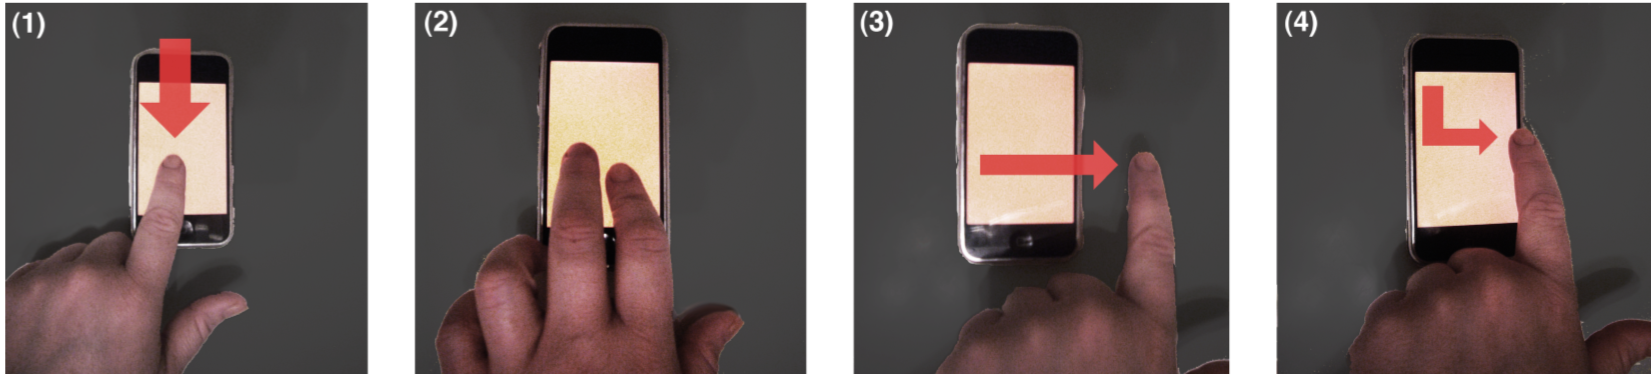
\includegraphics[width=4.5in]{slide-rule.jpg} 
\caption{An example of some multi-touch gestures recognized by Slide Rule.(1) A one-finger scan to browse lists; (2) A two-finger tap to select items; (3) A flick gesture used to flip between pages; (4) An L-select gesture to browse hierarchy of menu options. \cite{Kane:2008:SRM:1414471.1414487} }
\label{slide-rule}
\end{figure}

Slide Rule's design is ``based on interviews with blind mobile device users and on user-centered design with blind people.'' \cite{Kane:2008:SRM:1414471.1414487} The results from a study pertaining to the usability of Slide Rule showed that users were able to complete tasks more quickly with Slide Rule than with a button-based mobile screen reader. However, the users did make more errors. \cite{Kane:2008:SRM:1414471.1414487} 

Researchers have also explored techniques to address specific aspects of blind touch screen interaction such as text entry\cite{Tinwala:2010:ETE:1868914.1868972, Bonner:2010:NNA:2166616.2166649} and gesture selection.\cite{Kane:2011:UGB:1978942.1979001}

The significance of all of these proposed solutions is that they were each developed by researchers specifically to address the needs of Individuals with Blindness or Severe Visual Impairment. Many studies, including each study mentioned in this section, only tested how the solutions improved usability for IBSVI. The extent to which these solutions helped sighted users was not examined.
  

\subsection{Relevant Emerging Technology}
There exists some relevant emerging technology that makes touch screen devices more tactile. Though these emerging devices may not have been created with the usability limitation directly in mind, the devices still appear to be possible solutions to the problem at hand.

One noteworthy device comes from Tactus Technology, a company in Fremont, California. Employees from Tactus Technology are creating a keyboard with shape-shifting keys that pop up from the screen's surface when needed and recede again when no longer necessary.\cite{Tactus} Craig Ciesla, the co-founder of the company, said that the keyboard will be offered later this year. (see Figure~\ref{tactus-keyboard}).

\begin{figure}[ht]
\centering
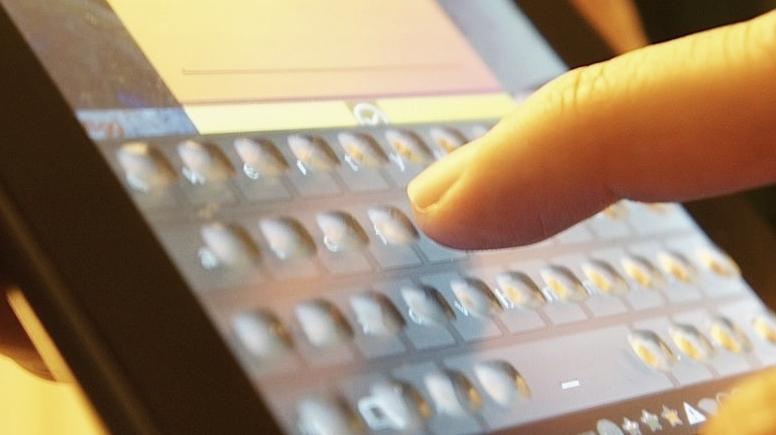
\includegraphics[width=3in]{tactus-keyboard.jpg} 
\caption{A Tactus keyboard}
\label{tactus-keyboard}
\end{figure}


\section{Discussion}
Prior work pertaining to the usability of touch screen devices has focused primarily on how Individuals with Blindness or Severe Visual Impairment (IBSVI) interact with the screens. Many proposed solutions to the lack of tactile feedback have been developed specifically for IBSVI. There also exist certain studies that examine usability of touch screen devices for sighted users. \cite{Tinwala:2010:ETE:1868914.1868972} However, there does not seem to be any research in the field that examines how tactile feedback affects usability for IBSVI \textit{and} sighted users alike.

Usability research evaluating touchscreen efficacy for both IBSVI and sighted users still needs to be covered in the literature. I completely agree that the lack of accessibility for IBSVI is a major issue with touchscreen devices. However, providing more tactile feedback can increase usability not just for IBSVI, but also for sighted users. In Donald Norman's book, \textit{The Design of Everyday Things}, Norman touches on this principle of feedback. Norman describes how telephones in the past ``were designed with much more care and concern for the user'' as ``the push buttons were designed to give an appropriate feel---tactile feedback.''\cite{Norman02} Norman asserts that modern telephone systems are ``so difficult to use'' since they have ``more features and less feedback.''\cite{Norman02} As tactile feedback is significant for IBSVI and sighted users alike, research should examine how both groups of users respond to proposed solutions. I think that this could possibly lead to a solution that becomes more widely accepted.



\section{Conclusions}
This study examined the usability of touchscreen devices by looking specifically at the limitation of the lack of tactile feedback. The literature focuses primarily on how this limitation reduces learnability and efficiency of touchscreen devices for Individuals with Blindness or Severe Visual Impairment. Many proposed solutions to this usability limitation are centered around the needs of IBSVI. Though there exist some studies pertaining to how this limitation affects usability for sighted users, the findings are not as comprehensive. There also exist a few devices that were not necessarily centered around the needs of IBSVI, such as the Tactus keyboard. The main concept missing from this field of study is solutions to the limitation that are effective for IBSVI and sighted users alike.

\clearpage

\bibliography{mybib}{}
\bibliographystyle{plain}
\end{document}

\end{document}
